\documentclass[12pt]{article}
\usepackage[utf8]{inputenc} % uft8 you know
\usepackage[danish]{babel}
\usepackage{lastpage}
\usepackage{fancyhdr}
\usepackage{hyperref}
\usepackage{comment}
\usepackage[backend=biber,style=apa,sorting=ynt]{biblatex}
\addbibresource{sources/library.bib}
\usepackage[T1]{fontenc}
\usepackage{ae}
\usepackage{graphicx}
\usepackage{array}
\usepackage{ragged2e} % for \RaggedRight command
\usepackage{booktabs} % for \toprule, \midrule, \bottomrule
\usepackage{pdfpages} % Til at inkludere pdf'er
\usepackage{amsmath}
\usepackage{amsfonts}
\usepackage{amssymb}
\usepackage{longtable}
\usepackage{adjustbox}
\usepackage{blindtext}
\usepackage{geometry}
\usepackage{xcolor}
\usepackage{soul}
\newcommand{\mathcolorbox}[2]{\colorbox{#1}{$\displaystyle #2$}}
\usepackage{multirow}
%\usepackage{natbib} % Works with.bib files
%\bibliographystyle{apalike} 
\usepackage{tabularx, booktabs, siunitx} % From now on ist only code styling!
% Default fixed font does not support bold face
\DeclareFixedFont{\ttb}{T1}{txtt}{bx}{n}{12} % for bold
\DeclareFixedFont{\ttm}{T1}{txtt}{m}{n}{12}  % for normal
% Custom colors
\usepackage{color}
\definecolor{deepblue}{rgb}{0,0,0.5}
\definecolor{deepred}{rgb}{0.6,0,0}
\definecolor{deepgreen}{rgb}{0,0.5,0}
\newcommand\pythonstyle{\lstset{
language=Python,
basicstyle=\ttm,
morekeywords={self},              % Add keywords here
keywordstyle=\ttb\color{deepblue},
emph={MyClass,__init__},          % Custom highlighting
emphstyle=\ttb\color{deepred},    % Custom highlighting style
stringstyle=\color{deepgreen},
frame=tb,                         % Any extra options here
showstringspaces=false,
breaklines=true
}}

\usepackage{hyperref}
\usepackage{caption}
\DeclareCaptionFont{white}{\color{white}}
\DeclareCaptionFormat{listing}{\colorbox{blue}{\parbox{\textwidth}{\hspace{15pt}#1#2#3}}}
\captionsetup[lstlisting]{format=listing,labelfont=white,textfont=white, singlelinecheck=false, margin=0pt, font={bf,footnotesize}}
\usepackage{listings}

\geometry{
    a4paper,
    total={170mm,257mm},
    left=20mm,
    top=30mm,
    bottom=30mm,
}
\hypersetup{
    linkcolor=black,
    colorlinks=false,
    pdftitle={Fysik eksammens forberedelse},
    pdfauthor={Kristoffer Sørensen}, % Obs: Din lokale kopi, skal indeholde dit navn og KUN dit navn. 
    % Remove the red border around links
    pdfborder={0 0 0},
}

\pagestyle{fancy} % definds the pagestyleing
\fancyhf{} % Removes the wired header text
\renewcommand{\headrulewidth}{0pt} % Removes the line under the header
\cfoot{Side \thepage\ af \pageref{LastPage}} % Sets the right side of the footer to "Page X of Y"
%\lhead{Gruppe 1} % Sets the left side of the header to "Gruppe 1"

\begin{document}
    \input{chapters/00TitlePage.tex}
    \newpage 
\part{Eksamensopgaver}
\section{Eksammens opgave 1 - Lys}\label{sec:Exam01}
%\subsection{God viden til afsnit: \ref{sec:Exam01}}
%\subsubsection{Fysiskestørelser}
%\begin{center}
    %\renewcommand{\arraystretch}{1.5}
    %\begin{tabular*}{\textwidth}{@{\extracolsep{\fill}} c l c}
        %\hline
        %Symbol & Navn af størrelse & Enhed \\
        %\hline
        %\begin{math}v\end{math} & bølgens udbredelseshastighed & \begin{math}m s^{-1}\end{math}\\
        %\begin{math}\lambda\end{math} & bølgelængde & m \\
        %\begin{math}f\end{math} & frekvens & Hz \\
        %\begin{math}T\end{math} & periode & s \\
       % \begin{math}I\end{math} & indfaldsvinkel & grader \\
      %  \begin{math}B\end{math} & brydningsvinkel & grader \\
     %   \begin{math}I_c\end{math} & kritisk vinkel & grader \\
    %    \begin{math}n_1\end{math} & brydningsindex 1 & 1 \\
   %     \begin{math}n_2\end{math} & brydningsindex 2 & 2 \\
  %      \hline
 %   \end{tabular*}
%\end{center}
\subsection{Beregn lysets frekvens i luft når bølgelængden er 560nm}
For at finde frem til frekvensen ved en bølgelængde på 560 nm må følgende formel anvendes:
\begin{equation*}
    v=\frac{\lambda}{T}
\end{equation*}
Vi ved, at perioden\begin{math}T\end{math} og frekvensen \begin{math}f\end{math} er relateret ved:
\begin{equation*}
    f=\frac{1}{T}
\end{equation*}
Dette betyder, at frekvensen er det inverse af perioden. Hvis perioden (\begin{math}T\end{math}) er lang, vil frekvensen (\begin{math}f\end{math}) være lav, og omvendt.\\\\
Hvis \begin{math}T\end{math} erstattes med \begin{math}\frac{1}{f}\end{math}
\begin{equation*}
    v=\frac{\lambda}{\frac{1}{f}}
\end{equation*}
For at få \begin{math}f\end{math} til at stå alene ganges der nu med \begin{math}1/f\end{math} på begge sider af lighedstegnet. 
\begin{equation*}
    v=\lambda \cdot f
\end{equation*}
For at finde frekvensen isoleres f på den ene side af lighedstegnet. Dette gøres ved at dividere med bølgelængden.
\begin{equation*}
    f=\frac{v}{\lambda}
\end{equation*}
Herefter indsættes værdierne i formlen og regnes ud. Det er opgivet at lysets hastighed er \begin{math}3,00 10^{8} m/s\end{math}. Og at lysets bølgelængde er 560 nm. Hvilket svarer til 560 x 10\textsuperscript{-9} m.
\begin{equation*}
    f=\frac{3,00 \cdot 10^{8} m/s}{560 \cdot 10^{-9} m}
\end{equation*}
Da m går ud med m så har man kun tilbage at:
\begin{equation*}
    f=5,36 \cdot 10^{14} s^{-1}
\end{equation*}
For at omskrive \begin{math}s^{-1}\end{math} til Hz anvender man det faktum at 1 Hz = 1 s\textsuperscript{-1}.
\textbf{\begin{equation*}
    \mathcolorbox{yellow}{f=5,36 \cdot 10^{14} Hz}
\end{equation*}}
% TODO: vurder om dette afsnit skal stå i teksen. En ting der er værd at vide er at \begin{math}v\end{math} også kendt som \begin{math}v_b\end{math} er bølgens udbredelseshastighed. Bølgens udbredelseshastighed er den hastighed, hvormed en bølge bevæger sig gennem et medium. 
\subsection{Beregn brydningsvinklen når indfaldsvinklen er 15. Lav en skite der ilustrerer brydningen}
For at finde frem til brydningsvinklen skal man bruge snells lov. Snells lov er en lov der beskriver hvordan lys brydes når det går fra et matriale til et andet. Brydningen skyldes hastighedsforskellen i de to materialer. Her er I indfaldsvinklen og B brydningsvinklen. 
\begin{equation*}
    \frac{sin(I)}{sin(B)}=\frac{n_2}{n_1}
\end{equation*}
Da man ønsker at finde brydningsvinklen ved 15 grader, skal man reducere udtrykket så man kan finden det rigtige udtryk for brydningsvinklen. Det gør man ved at isolere \begin{math}sin(B)\end{math} på den ene side af lighedstegnet. Det gøres ved at gange \begin{math}sin(B)\end{math} over på den anden side af lighedstegnet. 
\begin{equation*}
    sin(I)=sin(B) \cdot \frac{n_2}{n_1}
\end{equation*}
Herefter dividres med \begin{math}\frac{n_2}{n_1}\end{math} for at isolere \begin{math}sin(B)\end{math}
Så kommer det tilsidst til at se sådan her ud:
\begin{equation*}
    sin(B)=sin(I)\cdot\frac{n_1}{n_2}
\end{equation*}
Så indsættes værdierne i formlen og regnes ud. 
\begin{equation*}
    sin(B)=sin(15)\cdot\frac{1}{1.33}
\end{equation*}
\begin{equation*}
    sin(B)=0,1946
\end{equation*}
Så bruges invers sinus for at finde vinklen.
\begin{equation*}
    B=sin^{-1}(0,1946)
\end{equation*}
Dette giver en brydningsvinkel på 11 grader.
\begin{equation*}
    \mathcolorbox{yellow}{B=11^{\circ}}
\end{equation*}
\subsection{Find den kritiske vinkel hvor der totalreflektionen indtræffer}
Et nyt forsøg laves hvor lysstrålen sendes fra sprit op i luften. 
For at finde den kritiske vinkel skal man bruge følgende formel:
\begin{equation*}
    sin(I_c)=\frac{n_2}{n_1}
\end{equation*}
Her er \begin{math}I_c\end{math} den kritiske vinkel. \begin{math}n_2\end{math} er luftens brydningsindex og \begin{math}n_1\end{math} er sprits brydningsindex.
\begin{equation*}
    sin(I_c)=\frac{1}{1.36}
\end{equation*}
\begin{equation*}
    sin(I_c)=0.73529
\end{equation*}
\begin{equation*}
    I_c=sin^{-1}(0.73529)
\end{equation*}
\begin{equation*}
    \mathcolorbox{yellow}{I_c=47.3^{\circ}}
\end{equation*}
Altså vil der være totalreflektion når indfaldsvinklen er større end 47.3 grader.
\newpage
    \section{Atomfysik}
\subsection{Beregn energiniveauerne for skallerne n=2 og n=3}
For at finde frem til energiniveauerne for skallerne n=2 og n=3 skal man bruge den følgende formel:
\begin{equation*}
    E_n=-h\cdot c \cdot R \cdot \frac{1}{n^2}
\end{equation*}
Her er \begin{math}E_n\end{math} energiniveauet for den specefikke skal, \begin{math}h\end{math} er plancks konstant, \begin{math}c\end{math} er lysets hastighed, \begin{math}R\end{math} er Rydbergs konstant og \begin{math}n\end{math} er skallenummeret.
For at finde energiniveauet for skallen n=2 indsættes værdierne i formlen og regnes ud.
\begin{equation*}
    E_2=-6,63 \cdot 10^{-34} \frac{J}{s} \cdot 3 \cdot 10^8 m/s \cdot 1,097 \cdot 10^7 m^{-1}\cdot \frac{1}{2^2}
\end{equation*}
\begin{equation*}
    \mathcolorbox{yellow}{E_2=-5,45 \cdot 10^{-19} J}
\end{equation*}
\begin{equation*}
    E_3=-6,63 \cdot 10^{-34} frac{J}{s}  \cdot 3 \cdot 10^8 m/s \cdot 1,097 \cdot 10^7 m^{-1}\cdot \frac{1}{3^2}
\end{equation*}
\begin{equation*}
    \mathcolorbox{yellow}{E_3=-2,42 \cdot 10^{-19} J}
\end{equation*}
\subsubsection{Beregn energien for elektronovergangen fra 3 til 2}
For at finde energien for elektronovergangen fra 3 til 2 skal
\begin{equation*}
    E_{foton} = h \cdot f = E_n - E_m
\end{equation*}
Her er E\_n og E\_m energiniveauerne for de to skaller. h er plancks konstant og f er frekvensen.
\begin{equation*}
    E_{foton} = -5,45 \cdot 10^{-19} J - 2,42 \cdot 10^{-19} J
\end{equation*}
\begin{equation*}
    \mathcolorbox{yellow}{E_{foton} = -7,87 \cdot 10^{-19} J}
\end{equation*}

\subsection{Bestem frekvensen og bølgelængden af de fotoner der vil blive udsendt ved elektronovergangen}
For at finde bølgelængden af fotonen skal man bruge Rydbergs formel: 
\begin{equation*}
    \frac{1}{\lambda}=R \cdot (\frac{1}{n^2} - \frac{1}{m^2} )
\end{equation*}
Så skal lamda isoleres. 
\begin{equation*}
    \lambda = 1,097 \cdot 10^7 m^{-1} (\frac{1}{2^2} - \frac{1}{3^2} )
\end{equation*}
\begin{equation*}
    \mathcolorbox{yellow}{\lambda = 656 nm}
\end{equation*}
For at finde frekvensen kan man bruge formlen:
\begin{equation*}
    V=\frac{\lambda}{T}
\end{equation*}
Hvilket kan omskrives til 
\begin{equation*}
    V=\lambda \cdot f
\end{equation*}
Så isoleres f for at finde frekvensen.
\begin{equation*}
    f=\frac{V}{\lambda}
\end{equation*}
Så kan man indsætte værdierne i formlen og regne ud.
\begin{equation*}
    f=\frac{3 \cdot 10^8 m}{656 \cdot 10^{-9} m}
\end{equation*}
\begin{equation*}
    \mathcolorbox{yellow}{f=4,584 \cdot 10^{14} Hz}
\end{equation*}
\newpage

    \section{Eksamensopgave 3 - Varmelære}
\subsection{Beregn varmen der skal bruges til at opvarmningen af vandet når det varmes fra 10 grader til 100 grader}
For at finde den varme der kræves for at opvarme vandet fra 10 grader til 100 grader kan beskrives ved formlen: 
\begin{equation*}
    Q=m \cdot c \cdot \Delta T
\end{equation*}
Her er \begin{math}m\end{math} masssen, \begin{math}c\end{math} (\begin{math}
    \frac{J}{kg \cdot K}
\end{math}) er den specefikke varmekapacitet og $\Delta T$ er temperaturforskellen. Og Q er den varme der kræves (Joule)
For at finde massen skal man sige: 
\begin{equation*}
    m=\rho \cdot V
\end{equation*}
Her er $\rho$ densitet og V volumen.
\begin{equation*}
    m=997 \frac{kg}{m^3} \cdot 0,8 L
\end{equation*}
\begin{equation*}
    m=0,8 \cdot 10^{-3} m^3  \cdot 100 \frac{kg}{m^3}=0,08 kg
\end{equation*}
\begin{equation*}
    Q=0,8 kg \cdot 4180 \frac{J}{kg \cdot C} \cdot 90C
\end{equation*}
\begin{equation*}
    \mathcolorbox{yellow}{Q=301100 J}
\end{equation*}
\subsection{Beregn elkedlens nyttet virkning og forklar forskællen mellem energiforbruget og varmen der er tilført vandet.}
For at finde elkedlens nyttet virkning skal man bruge følgende formel: 
\begin{equation*}
    \eta=\frac{Q_{udnyttet}}{E_{tilført}}
\end{equation*}
Dog kan man ikke bare sætte tallene ind i formlen da man har fået givet den brugte energi i kwH og ikke i Joules. 
Derfor må man omregne det til Joules:
\begin{equation*}
    1 kWh=3,6 \cdot 10^6 J
\end{equation*}
Det vil sige at de 0,134 kWh er lig med:
\begin{equation*}
    0,134 kWh=0,134 kWh \cdot 3,6 \cdot 10^6 J
\end{equation*}
\begin{equation*}
    \mathcolorbox{yellow}{0,134 kWh=482400 J}
\end{equation*}
Nu kan der bare indsættes i formlen:
\begin{equation*}
    \eta=\frac{301100 J}{482400 J}\cdot 100
\end{equation*}
\begin{equation*}
    \mathcolorbox{yellow}{\eta=62\%}
\end{equation*}

\subsection{Beregn fællestemperaturen af tekanden og vandet når der er indtrådt termisk ligevægt}
For at finde fællestemperaturen skal man bruge følgende formel:
\begin{equation*}
    T_{fælles}= \frac{m_a \cdot C_a \cdot T_a + m_v c_v \cdot T_v}{m_g}
\end{equation*} % todo make fælles temperatur

\newpage
    \newpage
\section{Eksamensopgave 4 - Ellære}
\subsection{Beregn erstatningsresistansen i resistorkoblingen}
Når man beregner erstatningsresistansen i en resistorkobling, ønsker man at finde én enkelt resistor, som kan erstatte hele koblingen og have samme samlede modstand. Kan man starte med at finde de resistorer der sidder i parallelforbindelsen, og beregne deres erstatningsresistansen. 
I denne opgave skal i beregne modstanden for en parallel forbindelse som også har en serie forbindelse. Dog inden man gør det angiver man hvad man vil kalde ens modstande for ikke at der bilver forvirrene.\newline
\begin{figure}[h!]
    \centering
    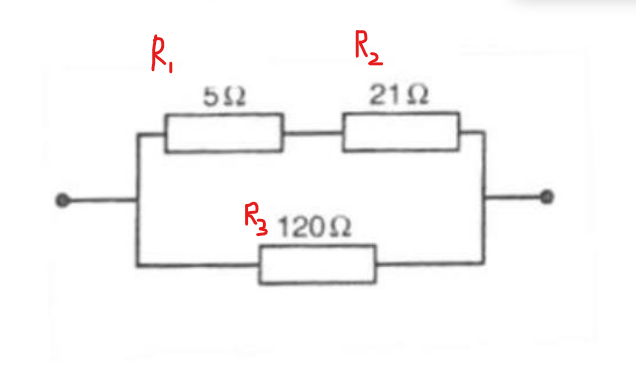
\includegraphics[width=0.5\textwidth]{figures/resistans.png}
    \caption{Indtegning af navne samt resistorkobling}
\end{figure}
Herefter skal man finde frem til værdien for den samlede erstatningsresistansen, da det er i en parallelforbindelsen anvendes formlen for en parallelforbindelse.
\begin{equation*} % TODO: Evt nævn at det er kirchhoffs 1. lov
    R_{12}=R_{1}+R_{2}
\end{equation*}
\begin{equation*}
    \mathcolorbox{yellow}{R=5\Omega+21\Omega=26\Omega}
\end{equation*}
Formlen for en parallel forbindelse ser sådan ud:
\begin{equation*}
    \frac{1}{R_{total}}=\frac{1}{R_{1}}+\frac{1}{R_{2}}
\end{equation*}
Da de er parallel skal man huske at tage den reciprokke værdi til sidst.
\begin{equation*}
    R_{total}=\left(\frac{1}{26\Omega}+\frac{1}{120\Omega}\right)^{-1}
\end{equation*}

\begin{equation*}
    \frac{1}{R_{total}}=\frac{1}{26\Omega}+\frac{1}{120\Omega}=0,04679\Omega^{-1}=\mathcolorbox{yellow}{21,37\Omega}
\end{equation*}

\subsection{Modstanden på 5~$\Omega$ laves af en kobbertråd med længden 60m. Bestem trådens radius.}
For at beregne kobbertrådens radius kan vi bruge følgende formel:
\begin{equation*}
    R=\rho\cdot\frac{l}{A}
\end{equation*}
$R$ = Modstand i ohm ~$\left[ \Omega \right]$\newline
    $\rho$ = Resistivitet for kobbertråden er den på $0,0155 \cdot 10^{-6} \Omega$ \newline
    $l$ = Længden af kobbertråden\newline
    $A$ = Tværsnitsarealet\newline

For at bruge denne formel skal vi have isoleret A, som vi gør ved at gange med A på begge sider og derefter dividere med R på begge sider. Derfor kommer formlen til at se sådan ud.
\begin{equation*}
    A=\frac{l\cdot\rho}{R}
\end{equation*}
Nu kan vi indsætte vores værdier
\begin{equation*}
    A=\frac{60m\cdot0,0155 \cdot 10^{-6} \Omega \cdot m}{5\Omega}
\end{equation*}
\begin{equation*}
    A = \frac{9,3 \cdot 10^{-7} \cdot \Omega \cdot m^{2}}{5 \Omega} = 1,86 \cdot 10^{-7} \cdot m^{2} \approx 0,186 \cdot mm^{2}
\end{equation*}
Man har nu tværsnitsarealet og kan nu beregne radiusen af tråden ved bruge af formlen for aralet af en cirkel.
\begin{equation*}
    A=\pi*r^{2}
\end{equation*}
For at få radiusen isoleret skal vi isolere r. Dette gør man ved at dividere med $\pi$.
\begin{equation*}
    \frac{A}{\pi}=r^{2}
\end{equation*}
\begin{equation*}
    r^{2}=\frac{A}{\pi}
\end{equation*}
Hvorefter man tager kvadratroden af dette for at finde radiusen.
\begin{equation*}
    r=\sqrt{\frac{A}{\pi}}
\end{equation*}
Værdierne kan nu indsættes.
\begin{equation*}
    r=\sqrt{\frac{0,186mm^{2}}{\pi}} = \mathcolorbox{yellow}{0,243 mm}
\end{equation*}

\subsection{Et batteri med hvilespændingen 1,4V og en indre modstand på 0,5~$\Omega$ tilsluttes resistorkoblingen. Skitser situationen og beregn polspændingen.}
\begin{equation*}
    U_{pol}=U_{hvile}-I\cdot R_{indre}
\end{equation*}
\begin{equation*}
    I_{total}=\frac{1,4V}{21,37\Omega+0,5\Omega}=0,064A
\end{equation*}

\begin{equation*}
    U_{pol}=1,4V-0,5\Omega\cdot 0,064A=1,368V
\end{equation*}
\newpage
    \newpage
\section{Eksamensopgave 5 - Kinematik}
\subsection{Beregn murstenens position efter 0,1s}
Først start med at identificer de kendte værdier:
\\\\
Startposition: 50 meter \newline
Start hastighed: 0 m/s (da den falder frit fra hvile position)\newline
Tid: 0,1 sekunder \newline
Tyngdeacceleration: \begin{math}9,82m/s^{2}\end{math}


\subsubsection{Brug den kinematiske formel for position}
Den generelle formel for position ved frit fald er:
\begin{equation*}
    \mathcolorbox{yellow}{s=1/2 \cdot g \cdot t^{2}}
\end{equation*}

\subsubsection{Indsæt værdierne i formlen og udregn}
\begin{equation*}
    \mathcolorbox{yellow}{1/2 \cdot 9,82m/s^{2} \cdot (0,1s)^{2}=0,0491m}
\end{equation*}

Murstenens position efter 0,1s er 49,95m

\subsection{Bestem hvor lang tid der går, inden murstenen rammer jorden}

Først identificer vi de kendte værdier som er brugt ovenover

\subsubsection{Brug den kinematiske formel for position}
\begin{equation*}
    \mathcolorbox{yellow}{1/2\cdot g\cdot t^{2}=s}
\end{equation*}
Indsæt værdierne
\begin{equation*}
    \mathcolorbox{yellow}{1/2\cdot9,82m/s^{2}\cdot t^{2}=50m}
\end{equation*}
Dette giver t = 3,191s. Hvilket betyder at der går 3,191s før murstenen rammer jorden.

\subsection{Beregn murstenens hastighed, lige inden den rammer jorden}
For at kunne udregne dett bruger vi formlen nedenunder.
\begin{equation*}
    \mathcolorbox{yellow}{v=a\cdot t}
\end{equation*}
\subsubsection{Indsæt de kendte værdier}
\begin{equation*}
    \mathcolorbox{yellow}{9,82m/s^{2}\cdot 3,191s = 31,34 m/s}
\end{equation*}


\newpage
    \newpage
\section{Eksamensopgave 7 - Gasser}
\subsection{Beregn tyngdekraften på ballon uden luft}
Først start med at skriver man de kendte værdier:
\\\\
Volume: \begin{math}3m^3\end{math} \newline
Vægt: \begin{math}0,110kg\end{math} \newline
Ved brug af newtons 2. lov \begin{math}F_{res}=m\cdot a\end{math} kan man udregne tyngdekraften på ballonen uden luft. \newline
Jordens tyngdeacceleration er ca. \begin{math}9,82 m/s^2\end{math} som kan også skrives som \begin{math}9,82N/kg\end{math} det varierer lidt i forhold til hvor på jorden man er. \newline

\begin{equation}
	F_t=0,110kg\cdot9,82 N/kg=1,08N
\end{equation}
\subsection{Skitser kræfterne der påvirker ballonen og beregn opdriften. Det kan antaages at tempraturen er 20 grader C og at densiteten for luften i lokalet dermed er \begin{math}\rho=1,20kg/m^3\end{math}}
Igen begynder vi med at skrive de brugbar værdier ned:
\\\\
Densiteten: \begin{math}1,20kg/m^3\end{math} \newline
Volume: \begin{math}3m^3\end{math} \newline
Ved brug af Archimedes' lov \begin{math}F_{op}=\rho\cdot V\cdot g\end{math}, kan man udregne opdriften der påvirker ballonen, tyngdeaccelerationen er stadig \begin{math}9,82 N/kg\end{math}
\begin{equation}
	F_{op}=1,20kg/m^3 \cdot 3m^3 \cdot 9,82N/kg=3,535N
\end{equation}


    \newpage
\section{Eksamensopgave 8 - Vekselsstrøm}
\subsection{Kurven viser spændingsvariationer på en strømforsyning. Bestem maksimalspænidng, effektivspænding og frekvens.}
\begin{figure}[h!]
    \centering
    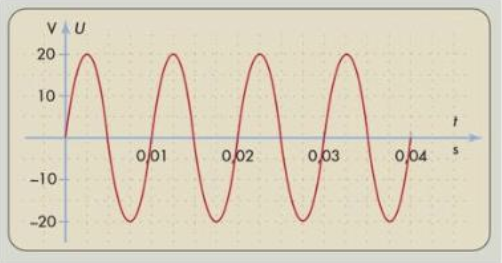
\includegraphics[width=0.5\textwidth]{figures/vekselsstrom.png}
    \caption{Kurve over vekselsstrøm}
\end{figure}
For at finde maks spænding \begin{math}U_{max}\end{math} kan vi kigge på den graf som vi har fået. På grafen kan vi se at den ikke går over 20V eller under 20V som betyder at maksimalspændingen er 20V\newline
For at finde effektivspænding kan vi bruge denne formel:
\begin{equation*}
    maximalspænding = \sqrt{2}\cdot effektivspænding
\end{equation*}
\begin{equation*}
    U_{max} = \sqrt{2}\cdot U_{eff}
\end{equation*}
Denne formel bruges til at finde maksimalspændingen med effektivspænding, men da vi allerede kender maksimalspændingen kan vi isolere effektivspænding ved at dividere med \begin{math}\sqrt{2}\end{math} på begge sider og beregne den ud fra den nye formel.
\begin{equation*}
    \frac{U_{maks}}{\sqrt{2}}=U_{eff}
\end{equation*}
\begin{equation*}
    U_{eff}=\frac{U_{maks}}{\sqrt{2}}
\end{equation*}
\begin{equation*}
    U_{eff}=\frac{20V}{\sqrt{2}}=14,14V
\end{equation*}
For at beregne frekvensen kan vi bruge denne formel
\begin{equation*}
    f=\frac{Antal Svingninger}{Tid}
\end{equation*}
På grafen kan vi se at den tager 1 svingning på 0,01 sekundt, derfor bliver formlen.
\begin{equation*}
    f=\frac{1}{0,01}=100Hz
\end{equation*}

\subsection{Spændingen tilkobles primærsiden på en transformer, der har 100 vindinger i primærspolen og 200 vindinger i sekundærspolen. Beregn spændingen på sekundærsiden.}
Til at beregne spændingen på sekundærsiden kan vi bruge denne formel
\begin{equation*}
    \frac{U_{s}}{U_{p}}=\frac{N_{s}}{N_{p}}
\end{equation*}
U står for spændingen\newline
N står for antal spoler\newline
S Står for sekundær\newline
P står for primær\newline
Med denne formel kan vi nu isolere \begin{math}U_{s}\end{math} ved at gange med \begin{math}U_{p}\end{math} på begge sider og indtaste værdierne.
\begin{equation*}
    U_{s}=U_{p}*\frac{N_{s}}{N_{p}}
\end{equation*}
\begin{equation*}
    U_{s}=20V*\frac{200}{100}=20V*2=40V
\end{equation*}

\subsection{Spændingen fra opgave a tilkobles en transmissionsledning på 100m med en modstand på 2,82 ohm. Der sendes 5 A gennem ledningen. Hvad bliver effekttabet i ledningen?}
\begin{equation*}
    P_{tab}=R\cdot I^{2}
\end{equation*}
\begin{equation*}
    P_{tab}=2,82\Omega\cdot 5^{2} A=2,82\Omega\cdot 25=70,5W
\end{equation*}

\newpage
    \newpage
\section{Eksamensopgave 9 - Gitter}
\subsection{Bestem gitterkonstanten}
Når vi skal beregne gitterkonstanten \begin{math}d\end{math} ved vi at på 1mm er der 300 spalter, derfor er formlen
\begin{equation*}
    d=\frac{1mm}{300 spalter} = 0,00333mm = 3,33 * 10^{-6} m
\end{equation*}


\subsection{Beregn afbøjningsvinklen \begin{math}\phi_{2}\end{math}}
For at beregne afbøjningsvinklen kan vi bruge denne formel.
\begin{equation*}
    sin(\phi)=\frac{n\cdot\lambda}{d}
\end{equation*}
\begin{math}\phi = vinkel\end{math} [deg]\newline
n = orden\newline
\begin{math}\lambda = bølgelængde\end{math} [m]\newline
d = gitterkonstant [m]\newline

\begin{equation*}
    sin(\phi_{2})=\frac{2\cdot 590\cdot 10^{-9}}{3,33\cdot 10^{-6}}
\end{equation*}
\begin{equation*}
    sin(\phi_{2})=0,354
\end{equation*}
\begin{equation*}
    \phi_{2}=sin^{-1}(0,354)=20,75^{\circ}
\end{equation*}
\subsection{Bestem antallet af ordner der kan ses}
For at beregne antallet af order der kas ses kan vi bruge denne formel.
\begin{equation*}
    n=\frac{d}{\lambda}
\end{equation*}
\begin{equation*}
    n=\frac{3,33\cdot 10^{-6}}{590\cdot 10^{-9}} = 5,64
\end{equation*}
Da man ikke kan se et orden med et kommatal som 0,64 skal vi runde ned til 5. Derfor er svaret at man kan se 5 ordner.

\newpage
    \newpage
\section{Eksamensopgave 10 - Det skrå kast}
\begin{figure}[h!]
    \centering
    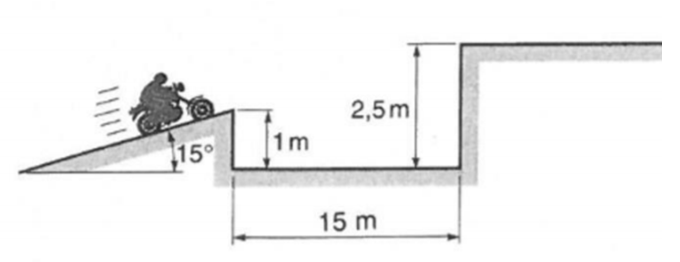
\includegraphics[width=0.5\textwidth]{figures/skrakast.png}
    \caption{Skrå kast opgave}
\end{figure}
\subsection{Hvor lang tid taget springet, når hastigheden er 30m/s}
For at beregne hvor lang tig sprinter tager skal vi først beregne \begin{math}v_{0x}\end{math}\newline
\begin{math}v_{0}\end{math} = Start hastigheden\newline
\begin{math}v_{0x}\end{math} = Start hastigheden på x-aksen\newline
\begin{math}y_{0}\end{math} = Start højde\newline
\begin{math}\alpha\end{math} = Start vinkel\newline
t = tid

\begin{equation*}
    v_{0x}=v_{0}\cdot cos(\alpha)
\end{equation*}
\begin{equation*}
    v_{0x}=30m/s\cdot cos(15^{\circ}) = 28,977 m/s
\end{equation*}
Nu når vi har \begin{math}v_{0x}\end{math} kan vi beregne tiden det tog.
\begin{equation*}
    x=v_{0}\cdot cos(\alpha)\cdot t
\end{equation*}
Nu skal t isoleres ved at dividere med \begin{math}v_{0x}\cdot cos(\alpha)\end{math} på begge sider.
\begin{equation*}
    \frac{x}{v_{0}\cdot \cos(\alpha)}=t
\end{equation*}
\begin{equation*}
    t=\frac{x}{v_{0}\cdot \cos(\alpha)}
\end{equation*}
Fra formlen før ved vi allerede at \begin{math}v_{0}\cdot cos(\alpha) = v_{0x} = 28,977m/s\end{math} og derfor kan formlen omskrives til
\begin{equation*}
    t=\frac{x}{v_{0x}}
\end{equation*}
\begin{equation*}
    t=\frac{15m}{28,977m/s} = 0,518 s
\end{equation*}



\subsection{Skitsér situationen i et koordinatsystem. Indtegn de kræfter som påvirker akrobaten.}
\begin{figure}[h!]
    \centering
    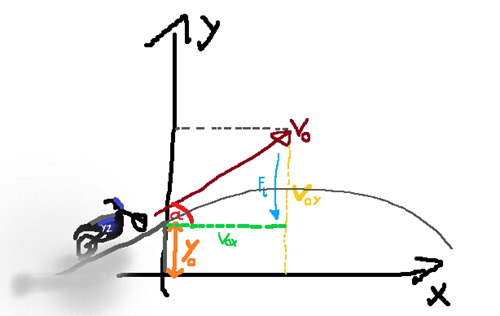
\includegraphics[width=0.8\textwidth]{figures/moterhop.png}
    \caption{Skitse af skrå kast opgave, med kræfterne indtegnet.}
\end{figure}

\subsection{Hvor højt passerer han over kanten, hvis farten ved afsættet er 100 km/t?}
Først skal vi omregne 100 km/t til m/s
\begin{equation*}
    v_{0}=\frac{100\cdot 1000}{3600}m/s = 27,78m/s
\end{equation*}
Nu kan vi beregne \begin{math}v_{0x}\end{math} og tiden på samme måde som i opgave a
\begin{equation*}
    v_{0x}=27,78m/s\cdot cos(15^{\circ}) = 26,82 m/s
\end{equation*}
\begin{equation*}
    t=\frac{15m}{26,82m/s} = 0,559 s
\end{equation*}

Nu skal vi beregne y værdien efter 0,559 sekunder med denne formlen
\begin{equation*}
    y_{slut} = -\frac{1}{2}\cdot g\cdot t^{2} + v_{0}\cdot sin(\alpha)\cdot t + y_{0}
\end{equation*}
\begin{equation*}
    y_{slut} = -\frac{1}{2}\cdot 9,82m/s^{2}\cdot 0,559^{2} s + 27,78\cdot sin(15)\cdot 0,559s + 1m = 3,48m
\end{equation*}
Nu har vi den totale højde på y-aksen, derfor skal vi minusse med \begin{math}2,5m - 1m\end{math} da det er højde forskellen, og så kan vi finde højden over kanten
\begin{equation*}
    y_{over} = 3,48m - 1,5m = 1,98m
\end{equation*}
\newpage
    %\newpage
    %\printbibliography[ heading=bibintoc, title={Litteratur}]
    %\input{chapters/99Bilag.tex}
\end{document}